\documentclass[11pt,fleqn]{article}
\usepackage{latexsym,epsf,epsfig}
\usepackage{amsmath,amsthm}
\usepackage{xy}
\input xy
\xyoption{all}
\begin{document}
\newcommand{\mbf}[1]{\mbox{{\bfseries #1}}}
\newcommand{\N}{\mbf{N}}
\renewcommand{\O}{\mbf{O}}

\noindent Bill Davis \\
Homework 4 

\begin{enumerate}
\item %Problem 1
If we have a second order Markov process, with Variables $X_{1}, X_{2} , X_{3} ...$, where $P(X_{t}|X_{0:t-1})$ $P(X_{t}|X_{t-1}X_{t-2})$ Then we can translate this to a new Markov Process with variables $Y_{1}=X_{1}X_{2}, Y_{2}=X_{2}X_{3}, Y_{3}=X_{3}X_{4}...$ where $P(Y_{t}|Y_{0:t-1})=P(Y_{t}|Y_{t-1})$
\item %Problem 2
The expected monetary value of each lottery ticket is 50 cents. \\
%U(S_{k}) < 49/50*U(S_{k-1}) + 1/50 * U(S_{k+10}) \\
%U(S_{k}) < 1999999/2000000*U(S_{k-1}) + 1/2000000 * U(S_{k+1000000})
\item %Problem 3
We can show this by observing that 
\[
VPI_{E}(E_{j}) = \displaystyle\sum_{k}P(E_{j}=e_{jk}|E)EU(\alpha_{jk}|E,E_{j}=e_{jk}) - EU(\alpha|e)
\]
Therefor so long as 
\[
\displaystyle\sum_{k}P(E_{j}=e_{jk}|E)EU(\alpha_{jk}|E,E_{j}=e_{jk}) >= EU(\alpha|e)
\]
VPI will be positive. We can show this by noting that, at the minimum if we don't change our action as a result of the new evidence, then the left hand side of the above equation is the sum over probabilities of the evidence node $E_{j}$. The sum of the probabalities of $E_{j}$ must equal 1. This means that 
\[
\displaystyle\sum_{k}P(E_{j}=e_{jk}|E)EU(\alpha|E,E_{j}=e_{jk}) = EU(\alpha|e)
\]
in the case where we don't change our action as a result of the new evidence. It follows that we may be able to change our action and increase our value. 

We can make a worse decision after receiving information because if we receive information that our selected action is terrible, but some previously identified lesser action is available we receive value not just from being able to take the lesser action, but being able to avoid our first (worse) action. 

\item %Problem 4
\begin{enumerate}
\item 
$R(s_{1})=1 +0.9*0.8*1 + 0.9*0.1*3+ 0.9*0.1*-1 = 1.9$\\
$R(s_{2})=3 +0.9*0.2*1 + 0.9*0.1*3+ 0.9*0.7*-1 = 2.82$\\
$R(s_{3})=-1 +0.9*0.9*1 + 0.9*0.1*3+ 0.9*0.0*-1 = 0.08$\\

\item 
$R(s_{1})=1 +0.1*0.8*1 + 0.1*0.1*3+ 0.1*0.1*-1 = 1.1$\\
$R(s_{2})=3 +0.1*0.2*1 + 0.1*0.1*3+ 0.1*0.7*-1 = 2.98$\\
$R(s_{3})=-1 +0.1*0.9*1 + 0.1*0.1*3+ 0.1*0.0*-1 = -0.88$\\
\item 

\end{enumerate}

\item %Problem 5
\begin{enumerate}
\item If we have a $V^{\pi}$ such that $\exists s$ where $V^{\pi}(s)>V^{*}(s)$, then we can construct a new $V^{**}$ where $V^{**}(s')=V^{*}(s')$ for all $s'\ne s$ and $V^{**}(s)=V^{\pi}(s)$. This $V^{**}$ is now optimal and not equal to $V^{*}$ which is a contradiction of the optimality of $V^{*}$.
\item 
If $\forall s V_{1}(s)<=V_{2}(s)$ then it naturally follows that $\forall s',a, s P((s'|s,a)V_{1}(s') < P((s'|s,a)V_{2}(s')$, since $P((s'|s,a) $ will be the same regardless of which V is in effect. Therefor
 $\sum_{s'\in S}  P((s'|s,a)V_{1}(s') < \sum_{s'\in S} P((s'|s,a)V_{2}(s')$ and we have shonw that $B(V_{1})<B(V_{2})$ 
\item 

\end{enumerate}
\item %Problem 6
\begin{enumerate}
\item $\beta < 2\alpha$
\item $\beta<\frac{1}{2} \alpha +\frac{\pi}{2}$

\item 
%\begin{figure}[h]
%\begin{center}
%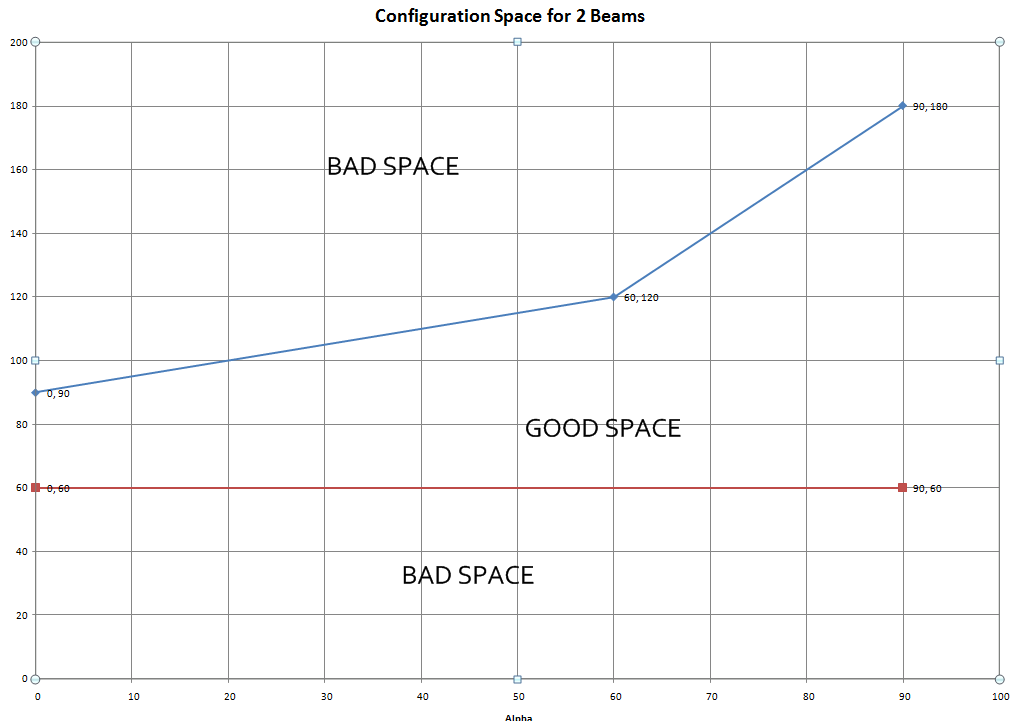
\includegraphics[height=80mm]{configurationspace.png}`
%\caption{Configuration Space for Problem 6c}
%\end{center}
%\end{figure}

Here the area between the two lines is good configuration space, everything else is bad. The Lower line represents the problem that $\beta$ cannot go to zero on account of the right hand wall. 
\end{enumerate}
\item %Problem 7
\begin{enumerate}
\item
Generate an empty map of the environment.  \\ 
Mark the center of the map explored. \\
Select the nearest unexplored node, where nearest is defined as a node adjacent to explored space. If there are multiple spaces, select one at random. Use Value-Iteration to generate a policy to  get from the current position to the unexplored node. \\
Continue until the goal is reached.\\

This works because we will always have a path from the current position to the unexplored node
\item 
Move Foward until a wall is encountered. Then move randomly move either counter-clockwise or clockwise until a free direction is available. Then move in that direction. 

This is not guaranteed to allow the robot to reach the goal. 
\item 
The first algorithm will be not handle continuous state space, but could be managed by discretizing the space. It will have problems with noise, but by switching to on-line QLearning as opposed to Value-Iteration the noise model could be learned and managed. Unknown goal location is not relevent. And moving obstacles will be a problem because the map will no longer be valid, although the Q-Learning may be able to deal with that.

The reactive controller may be slightly bothered by noise, if it detects walls where there are none, but otherwise will be uneffected by the changes. 

\end{enumerate}

\item %Problem 8
\begin{enumerate}
\item 
Clearly there are a number of possible threats from AI technology. Intelligent machines could decide to wipe out the human race, as has been described in so many science fiction movies. It could potentially render human thought irrelevant, what could a human being create that a machine could not? What competetion can humans be for machines? Already they are better then us at most games. In the few instances where they are not, they are likely to become better, and rapidly surpase humans. I think there is also the potential for these intelligent machine to become misguided. Will self-aware machines have the same moral compass that humans seem to possess?

However for all the fears there are about intelligent machines, I feel they pose no real threat to humanity. They'll be bound by whatever restrictions are placed upon mankind, economic, physical and computational. Will intelligent machines be able to compute solutions to NP-Complete problems? Probably not. But as machines become more intelligent they'll have many things to offer in terms of the sciences and I think they'll contribute to a great many discoveries, discoveries that human minds would have been hard pressed to find. Additionally, just because humans seem to be limited in their intelligent, as evidenced that our brains are required to fit inside our skull, I think many future advances will result from the intermingling of humans and machines. Maybe in the future there won't be a clear cut distinction between what is machine intelligence and what is human. 
\item 
Regarding the possability of ultra-intelligent machines, I suppose I believe in their inevitability. Once nature proves something is possible, there is no stopping human beings from imitating it. There are countless examples of this, but I think the most appropriate is flight. Would we be building airplanes if had never seen a bird? I would argue not, and as evidenced by our own intelligence, self-consciousness is possible. Even if we had to build a machine which emulated the physically activity of a billion neurons, we will sooner or later create an aritificial intelligence. Does this make them too possible? Perhaps, but I definitely do not believe that true intelligent machines, at least as intelligent as we are, are impossible to build. 

I suppose its not a contradiction to both believe AI is impossible and also to think that it is a threat. Even if we never get truely intelligent machines, we have proven to some extent that machines can surpass humans at some tasks. This is evidenced in protections some on-line poker sites take against robot poker players. Although no one would argue that a poker playing AI agent is truely intelligent, it does pose a threat if you are playing poker against it. 
\end{enumerate}

\end{enumerate}

\end{document}
